\documentclass{standalone}
\usepackage{tikz}
\usetikzlibrary{patterns, positioning}


\begin{document}
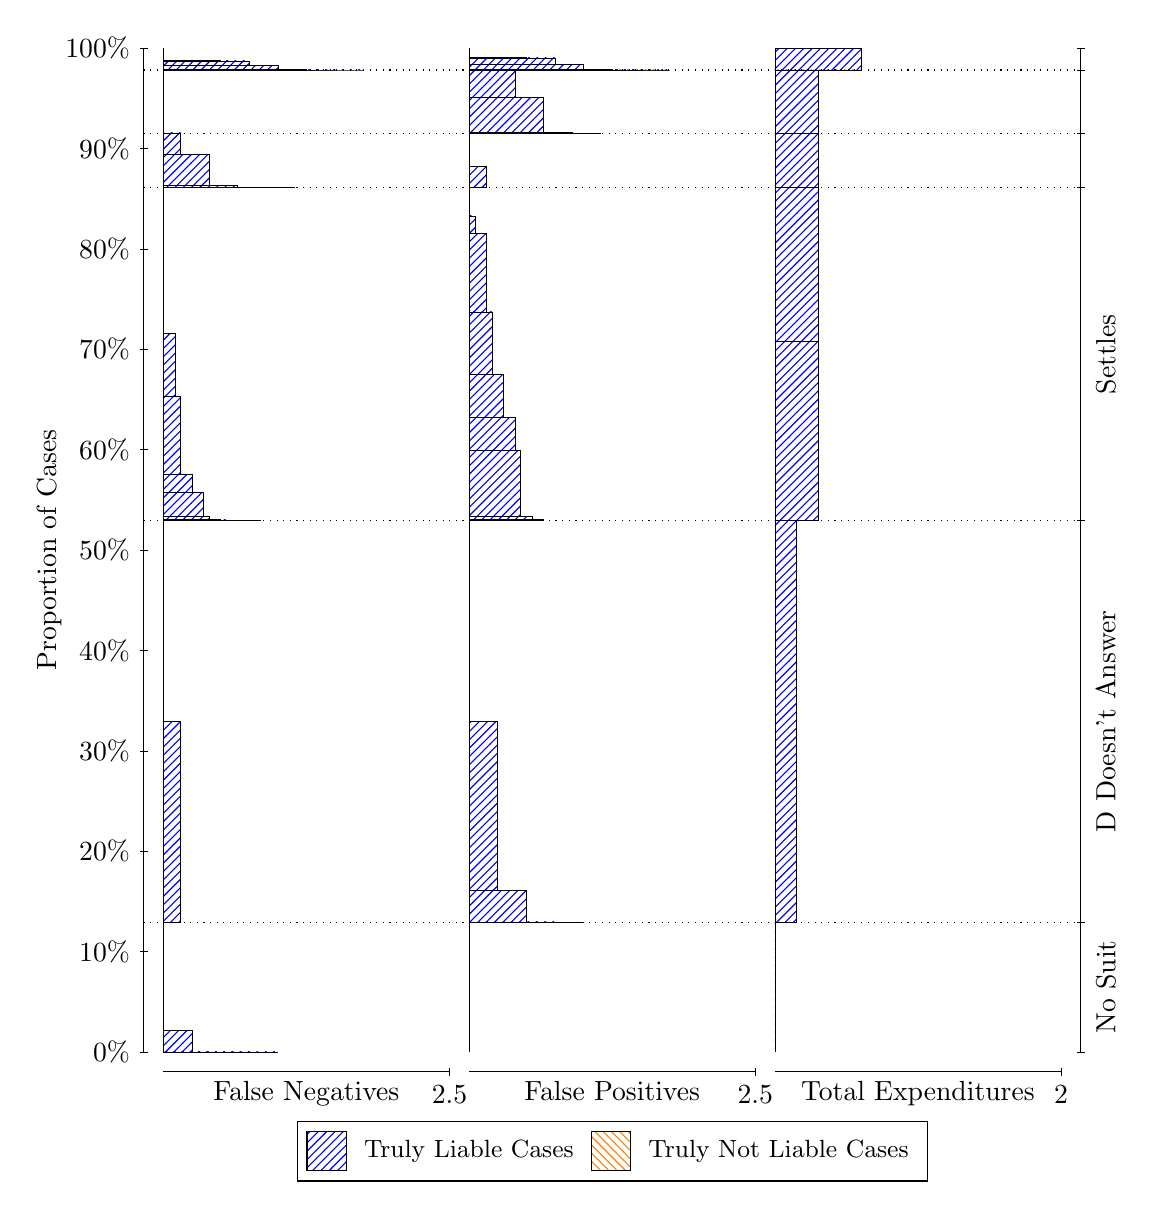
\begin{tikzpicture}
\draw[black, very thin] (1.5,1.75) -- (1.5,14.5);
\node[rotate=90, text=black, anchor=center] at (0.3, 8.125) {Proportion of Cases};
\draw[black, very thin] (1.45,1.75) -- (1.55,1.75);
\node[text=black, anchor=east] at (1.45, 1.75) {0\%};
\draw[black, very thin] (1.45,3.025) -- (1.55,3.025);
\node[text=black, anchor=east] at (1.45, 3.025) {10\%};
\draw[black, very thin] (1.45,4.3) -- (1.55,4.3);
\node[text=black, anchor=east] at (1.45, 4.3) {20\%};
\draw[black, very thin] (1.45,5.575) -- (1.55,5.575);
\node[text=black, anchor=east] at (1.45, 5.575) {30\%};
\draw[black, very thin] (1.45,6.85) -- (1.55,6.85);
\node[text=black, anchor=east] at (1.45, 6.85) {40\%};
\draw[black, very thin] (1.45,8.125) -- (1.55,8.125);
\node[text=black, anchor=east] at (1.45, 8.125) {50\%};
\draw[black, very thin] (1.45,9.4) -- (1.55,9.4);
\node[text=black, anchor=east] at (1.45, 9.4) {60\%};
\draw[black, very thin] (1.45,10.675) -- (1.55,10.675);
\node[text=black, anchor=east] at (1.45, 10.675) {70\%};
\draw[black, very thin] (1.45,11.95) -- (1.55,11.95);
\node[text=black, anchor=east] at (1.45, 11.95) {80\%};
\draw[black, very thin] (1.45,13.225) -- (1.55,13.225);
\node[text=black, anchor=east] at (1.45, 13.225) {90\%};
\draw[black, very thin] (1.45,14.5) -- (1.55,14.5);
\node[text=black, anchor=east] at (1.45, 14.5) {100\%};

\draw[black, very thin] (13.4,1.75) -- (13.4,14.5);
\draw[black, very thin] (13.35,1.75) -- (13.45,1.75);
\node[anchor=west] at (13.35, 1.75) {};
\draw[black, very thin] (13.35,3.3995) -- (13.45,3.3995);
\node[anchor=west] at (13.35, 3.3995) {};
\draw[black, very thin] (13.35,8.4975) -- (13.45,8.4975);
\node[anchor=west] at (13.35, 8.4975) {};
\draw[black, very thin] (13.35,12.727) -- (13.45,12.727);
\node[anchor=west] at (13.35, 12.727) {};
\draw[black, very thin] (13.35,13.418) -- (13.45,13.418);
\node[anchor=west] at (13.35, 13.418) {};
\draw[black, very thin] (13.35,14.221) -- (13.45,14.221);
\node[anchor=west] at (13.35, 14.221) {};
\draw[black, very thin] (13.35,14.5) -- (13.45,14.5);
\node[anchor=west] at (13.35, 14.5) {};

\draw[black, very thin, pattern color=blue, pattern=north east lines] (1.75,1.75) rectangle (3.2033,1.75);
\draw[black, very thin, pattern color=blue, pattern=north east lines] (1.75,1.75) rectangle (2.84,1.75);
\draw[black, very thin, pattern color=blue, pattern=north east lines] (1.75,1.75) rectangle (2.4767,1.7523);
\draw[black, very thin, pattern color=blue, pattern=north east lines] (1.75,1.7523) rectangle (2.1133,2.0201);
\draw[black, very thin, pattern color=orange, pattern=north west lines] (1.75,2.0201) rectangle (1.75,2.0201);
\draw[black, very thin, pattern color=blue, pattern=north east lines] (1.75,2.0201) rectangle (1.75,3.3995);
\draw[black, very thin, pattern color=blue, pattern=north east lines] (1.75,3.3995) rectangle (1.968,5.9453);
\draw[black, very thin, pattern color=orange, pattern=north west lines] (1.75,5.9453) rectangle (1.75,5.9453);
\draw[black, very thin, pattern color=blue, pattern=north east lines] (1.75,5.9453) rectangle (1.75,8.4975);
\draw[black, very thin, pattern color=blue, pattern=north east lines] (1.75,8.4975) rectangle (2.9853,8.4976);
\draw[black, very thin, pattern color=blue, pattern=north east lines] (1.75,8.4976) rectangle (2.84,8.4976);
\draw[black, very thin, pattern color=blue, pattern=north east lines] (1.75,8.4976) rectangle (2.6947,8.4976);
\draw[black, very thin, pattern color=blue, pattern=north east lines] (1.75,8.4976) rectangle (2.622,8.5066);
\draw[black, very thin, pattern color=blue, pattern=north east lines] (1.75,8.5066) rectangle (2.4767,8.5099);
\draw[black, very thin, pattern color=blue, pattern=north east lines] (1.75,8.5099) rectangle (2.3313,8.5529);
\draw[black, very thin, pattern color=blue, pattern=north east lines] (1.75,8.5529) rectangle (2.2587,8.8567);
\draw[black, very thin, pattern color=blue, pattern=north east lines] (1.75,8.8567) rectangle (2.1133,9.0805);
\draw[black, very thin, pattern color=blue, pattern=north east lines] (1.75,9.0805) rectangle (1.968,10.076);
\draw[black, very thin, pattern color=blue, pattern=north east lines] (1.75,10.076) rectangle (1.8953,10.872);
\draw[black, very thin, pattern color=orange, pattern=north west lines] (1.75,10.872) rectangle (1.75,10.872);
\draw[black, very thin, pattern color=blue, pattern=north east lines] (1.75,10.872) rectangle (1.75,12.727);
\draw[black, very thin, pattern color=blue, pattern=north east lines] (1.75,12.727) rectangle (3.4213,12.727);
\draw[black, very thin, pattern color=blue, pattern=north east lines] (1.75,12.727) rectangle (3.058,12.727);
\draw[black, very thin, pattern color=blue, pattern=north east lines] (1.75,12.727) rectangle (2.6947,12.756);
\draw[black, very thin, pattern color=blue, pattern=north east lines] (1.75,12.756) rectangle (2.3313,13.146);
\draw[black, very thin, pattern color=blue, pattern=north east lines] (1.75,13.146) rectangle (1.968,13.418);
\draw[black, very thin, pattern color=orange, pattern=north west lines] (1.75,13.418) rectangle (1.75,13.418);
\draw[black, very thin, pattern color=blue, pattern=north east lines] (1.75,13.418) rectangle (1.968,13.422);
\draw[black, very thin, pattern color=orange, pattern=north west lines] (1.75,13.422) rectangle (1.75,13.422);
\draw[black, very thin, pattern color=blue, pattern=north east lines] (1.75,13.422) rectangle (1.75,14.221);
\draw[black, very thin, pattern color=blue, pattern=north east lines] (1.75,14.221) rectangle (4.2933,14.221);
\draw[black, very thin, pattern color=blue, pattern=north east lines] (1.75,14.221) rectangle (3.93,14.221);
\draw[black, very thin, pattern color=blue, pattern=north east lines] (1.75,14.221) rectangle (3.5667,14.224);
\draw[black, very thin, pattern color=blue, pattern=north east lines] (1.75,14.224) rectangle (3.2033,14.282);
\draw[black, very thin, pattern color=blue, pattern=north east lines] (1.75,14.282) rectangle (2.84,14.338);
\draw[black, very thin, pattern color=blue, pattern=north east lines] (1.75,14.338) rectangle (2.622,14.338);
\draw[black, very thin, pattern color=blue, pattern=north east lines] (1.75,14.338) rectangle (2.4767,14.339);
\draw[black, very thin, pattern color=blue, pattern=north east lines] (1.75,14.339) rectangle (2.2587,14.339);
\draw[black, very thin, pattern color=blue, pattern=north east lines] (1.75,14.339) rectangle (2.2587,14.339);
\draw[black, very thin, pattern color=blue, pattern=north east lines] (1.75,14.339) rectangle (2.1133,14.339);
\draw[black, very thin, pattern color=blue, pattern=north east lines] (1.75,14.339) rectangle (1.8953,14.34);
\draw[black, very thin, pattern color=blue, pattern=north east lines] (1.75,14.34) rectangle (1.8953,14.346);
\draw[black, very thin, pattern color=orange, pattern=north west lines] (1.75,14.346) rectangle (1.75,14.346);
\draw[black, very thin, pattern color=blue, pattern=north east lines] (1.75,14.346) rectangle (1.75,14.5);
\draw[black, very thin, pattern color=orange, pattern=north west lines] (5.6333,1.75) rectangle (5.6333,1.75);
\draw[black, very thin, pattern color=blue, pattern=north east lines] (5.6333,1.75) rectangle (5.6333,3.3995);
\draw[black, very thin, pattern color=orange, pattern=north west lines] (5.6333,3.3995) rectangle (7.0867,3.3995);
\draw[black, very thin, pattern color=blue, pattern=north east lines] (5.6333,3.3995) rectangle (7.0867,3.3995);
\draw[black, very thin, pattern color=blue, pattern=north east lines] (5.6333,3.3995) rectangle (6.7233,3.4026);
\draw[black, very thin, pattern color=blue, pattern=north east lines] (5.6333,3.4026) rectangle (6.36,3.8068);
\draw[black, very thin, pattern color=blue, pattern=north east lines] (5.6333,3.8068) rectangle (5.9967,5.9517);
\draw[black, very thin, pattern color=blue, pattern=north east lines] (5.6333,5.9517) rectangle (5.6333,8.4975);
\draw[black, very thin, pattern color=orange, pattern=north west lines] (5.6333,8.4975) rectangle (6.578,8.4975);
\draw[black, very thin, pattern color=blue, pattern=north east lines] (5.6333,8.4975) rectangle (6.578,8.5117);
\draw[black, very thin, pattern color=orange, pattern=north west lines] (5.6333,8.5117) rectangle (6.4327,8.5117);
\draw[black, very thin, pattern color=blue, pattern=north east lines] (5.6333,8.5117) rectangle (6.4327,8.5554);
\draw[black, very thin, pattern color=orange, pattern=north west lines] (5.6333,8.5554) rectangle (6.2873,8.5554);
\draw[black, very thin, pattern color=blue, pattern=north east lines] (5.6333,8.5554) rectangle (6.2873,9.3941);
\draw[black, very thin, pattern color=blue, pattern=north east lines] (5.6333,9.3941) rectangle (6.2147,9.8046);
\draw[black, very thin, pattern color=blue, pattern=north east lines] (5.6333,9.8046) rectangle (6.0693,10.352);
\draw[black, very thin, pattern color=blue, pattern=north east lines] (5.6333,10.352) rectangle (5.924,11.148);
\draw[black, very thin, pattern color=blue, pattern=north east lines] (5.6333,11.148) rectangle (5.8513,12.144);
\draw[black, very thin, pattern color=blue, pattern=north east lines] (5.6333,12.144) rectangle (5.706,12.368);
\draw[black, very thin, pattern color=blue, pattern=north east lines] (5.6333,12.368) rectangle (5.6333,12.727);
\draw[black, very thin, pattern color=orange, pattern=north west lines] (5.6333,12.727) rectangle (5.8513,12.727);
\draw[black, very thin, pattern color=blue, pattern=north east lines] (5.6333,12.727) rectangle (5.8513,12.998);
\draw[black, very thin, pattern color=blue, pattern=north east lines] (5.6333,12.998) rectangle (5.6333,13.418);
\draw[black, very thin, pattern color=orange, pattern=north west lines] (5.6333,13.418) rectangle (7.3047,13.418);
\draw[black, very thin, pattern color=blue, pattern=north east lines] (5.6333,13.418) rectangle (7.3047,13.418);
\draw[black, very thin, pattern color=blue, pattern=north east lines] (5.6333,13.418) rectangle (6.9413,13.428);
\draw[black, very thin, pattern color=blue, pattern=north east lines] (5.6333,13.428) rectangle (6.578,13.87);
\draw[black, very thin, pattern color=blue, pattern=north east lines] (5.6333,13.87) rectangle (6.2147,14.216);
\draw[black, very thin, pattern color=blue, pattern=north east lines] (5.6333,14.216) rectangle (5.8513,14.221);
\draw[black, very thin, pattern color=orange, pattern=north west lines] (5.6333,14.221) rectangle (8.1767,14.221);
\draw[black, very thin, pattern color=blue, pattern=north east lines] (5.6333,14.221) rectangle (8.1767,14.221);
\draw[black, very thin, pattern color=orange, pattern=north west lines] (5.6333,14.221) rectangle (7.8133,14.221);
\draw[black, very thin, pattern color=blue, pattern=north east lines] (5.6333,14.221) rectangle (7.8133,14.221);
\draw[black, very thin, pattern color=orange, pattern=north west lines] (5.6333,14.221) rectangle (7.45,14.221);
\draw[black, very thin, pattern color=blue, pattern=north east lines] (5.6333,14.221) rectangle (7.45,14.227);
\draw[black, very thin, pattern color=orange, pattern=north west lines] (5.6333,14.227) rectangle (7.0867,14.227);
\draw[black, very thin, pattern color=blue, pattern=north east lines] (5.6333,14.227) rectangle (7.0867,14.291);
\draw[black, very thin, pattern color=blue, pattern=north east lines] (5.6333,14.291) rectangle (6.7233,14.374);
\draw[black, very thin, pattern color=blue, pattern=north east lines] (5.6333,14.374) rectangle (6.36,14.381);
\draw[black, very thin, pattern color=orange, pattern=north west lines] (5.6333,14.381) rectangle (6.142,14.381);
\draw[black, very thin, pattern color=blue, pattern=north east lines] (5.6333,14.381) rectangle (6.142,14.381);
\draw[black, very thin, pattern color=blue, pattern=north east lines] (5.6333,14.381) rectangle (5.9967,14.381);
\draw[black, very thin, pattern color=orange, pattern=north west lines] (5.6333,14.381) rectangle (5.7787,14.381);
\draw[black, very thin, pattern color=blue, pattern=north east lines] (5.6333,14.381) rectangle (5.7787,14.382);
\draw[black, very thin, pattern color=orange, pattern=north west lines] (5.6333,14.382) rectangle (5.6333,14.382);
\draw[black, very thin, pattern color=blue, pattern=north east lines] (5.6333,14.382) rectangle (5.6333,14.5);
\draw[black, very thin, pattern color=orange, pattern=north west lines] (9.5167,1.75) rectangle (9.5167,1.75);
\draw[black, very thin, pattern color=blue, pattern=north east lines] (9.5167,1.75) rectangle (9.5167,3.3995);
\draw[black, very thin, pattern color=orange, pattern=north west lines] (9.5167,3.3995) rectangle (9.7892,3.3995);
\draw[black, very thin, pattern color=blue, pattern=north east lines] (9.5167,3.3995) rectangle (9.7892,8.4975);
\draw[black, very thin, pattern color=orange, pattern=north west lines] (9.5167,8.4975) rectangle (10.062,8.4975);
\draw[black, very thin, pattern color=blue, pattern=north east lines] (9.5167,8.4975) rectangle (10.062,10.779);
\draw[black, very thin, pattern color=orange, pattern=north west lines] (9.5167,10.779) rectangle (10.062,10.779);
\draw[black, very thin, pattern color=blue, pattern=north east lines] (9.5167,10.779) rectangle (10.062,12.727);
\draw[black, very thin, pattern color=orange, pattern=north west lines] (9.5167,12.727) rectangle (10.062,12.727);
\draw[black, very thin, pattern color=blue, pattern=north east lines] (9.5167,12.727) rectangle (10.062,13.418);
\draw[black, very thin, pattern color=orange, pattern=north west lines] (9.5167,13.418) rectangle (10.062,13.418);
\draw[black, very thin, pattern color=blue, pattern=north east lines] (9.5167,13.418) rectangle (10.062,14.221);
\draw[black, very thin, pattern color=orange, pattern=north west lines] (9.5167,14.221) rectangle (10.607,14.221);
\draw[black, very thin, pattern color=blue, pattern=north east lines] (9.5167,14.221) rectangle (10.607,14.5);
\draw[black, dotted] (1.5,3.3995) -- (13.4,3.3995);
\draw[black, dotted] (1.5,8.4975) -- (13.4,8.4975);
\draw[black, dotted] (1.5,12.727) -- (13.4,12.727);
\draw[black, dotted] (1.5,13.418) -- (13.4,13.418);
\draw[black, dotted] (1.5,14.221) -- (13.4,14.221);
\draw[black, very thin] (1.75,1.5) -- (5.3833,1.5);
\node[text=black, anchor=north] at (3.5667, 1.5) {False Negatives};
\draw[black, very thin] (5.3833,1.45) -- (5.3833,1.55);
\node[text=black, anchor=north] at (5.3833, 1.45) {2.5};

\draw[black, very thin] (5.6333,1.5) -- (9.2667,1.5);
\node[text=black, anchor=north] at (7.45, 1.5) {False Positives};
\draw[black, very thin] (9.2667,1.45) -- (9.2667,1.55);
\node[text=black, anchor=north] at (9.2667, 1.45) {2.5};

\draw[black, very thin] (9.5167,1.5) -- (13.15,1.5);
\node[text=black, anchor=north] at (11.333, 1.5) {Total Expenditures};
\draw[black, very thin] (13.15,1.45) -- (13.15,1.55);
\node[text=black, anchor=north] at (13.15, 1.45) {2};

\node[text=black, centered, rotate=90] at (13.72, 2.5748) {No Suit};
\node[text=black, centered, rotate=90] at (13.72, 5.9485) {D Doesn't Answer};
\node[text=black, centered, rotate=90] at (13.72, 10.612) {Settles};




\draw (7.449999999999999,1.5) node[draw=none] (baseCoordinate) {};
\begin{scope}[align=center]
        \matrix[scale=0.5, draw=black, below=0.5cm of baseCoordinate, nodes={draw}, column sep=0.1cm]{
            \node[rectangle, draw, minimum width=0.5cm, minimum height=0.5cm, pattern color=blue, pattern=north east lines] {}; &
            \node[draw=none, font=\small, text=black] (B) {Truly Liable Cases}; &
            \node[rectangle, draw, minimum width=0.5cm, minimum height=0.5cm, pattern color=orange, pattern=north west lines] {}; &
            \node[draw=none, font=\small, text=black] (B) {Truly Not Liable Cases}; \\
            };
\end{scope}

\end{tikzpicture}
\end{document}